
%(BEGIN_QUESTION)
% Copyright 2006, Tony R. Kuphaldt, released under the Creative Commons Attribution License (v 1.0)
% This means you may do almost anything with this work of mine, so long as you give me proper credit

A pressure calibration device called a {\it deadweight tester} generates very precise pressures by means of calibrated weights placed on top of a hydraulic piston:

$$\includegraphics[width=15.5cm]{i00153x01.eps}$$

The secondary piston is moved in and out by turning a handle on a threaded rod.  Its sole purpose is to displace enough oil to force the primary piston to rise from its resting position, so that it is entirely suspended by oil pressure.  In that condition, the gauge will be subject to whatever pressure is proportional to the weights placed on top of the primary piston, and the area of the primary piston.

What will happen to the gauge's indication if the secondary piston is pushed in further?  What will happen to the gauge's indication if the secondary piston is pulled out, but not so far that the primary piston comes down to its resting position?  In other words, what effect does the secondary piston {\it position} have on pressure applied to the gauge?

$$\includegraphics[width=15.5cm]{i00153x02.eps}$$

\vskip 20pt \vbox{\hrule \hbox{\strut \vrule{} {\bf Suggestions for Socratic discussion} \vrule} \hrule}

\begin{itemize}
\item{} Why are deadweight testers considered accurate {\it standards} for fluid pressure?  What is it about their design and operation that makes them so accurate?  Conversely, what aspects of their construction would have to change in order to corrupt their inherent accuracy?
\item{} If a technician changes the type of fluid used in a deadweight tester (for example, from one type of oil to another), will its accuracy change?
\item{} Identify some potential problems one might encounter when using a deadweight tester.  What things, specifically, do you see that could go wrong with this device?
\end{itemize}

\underbar{file i00153}
%(END_QUESTION)





%(BEGIN_ANSWER)

Ideally, the secondary piston's position will have {\it no effect} on the oil pressure sent to the gauge.  Consequently, the gauge indication should not change.

%(END_ANSWER)





%(BEGIN_NOTES)

So long as the primary piston is completely suspended by oil pressure, the oil pressure {\it must} be equal to the force created by the weights (which does not change) divided by the area of the primary piston (which also does not change).  All the secondary piston does is displace oil to make the primary piston rise or fall.  It cannot ``miscalibrate'' the output of the tester, so long as the primary piston is kept suspended by oil and is not resting on anything that would take some of the weight and thus relieve the oil of any pressure.  Another way of saying this is that the output pressure of a deadweight tester is either spot-on or way off, and it is easy to tell when the pressure is not correct.

Practically, to check for primary piston binding, the primary piston is gently rotated as the secondary piston is pushed in.  When the primary piston is completely suspended by oil, it should rotate freely, the mass of the calibrating weights ensuring a long ``coasting'' time.  Slow rotation of the primary piston will overcome static friction, and allows the piston to settle in the position where it is most free.

I strongly recommend you bring an actual deadweight tester to class for live demonstration, preferably with a pressure gauge attached.  

\vskip 10pt

A common misconception among students is that a deadweight tester measures pressure.  Not so!  A deadweight tester {\it generates} precisely accurate pressures to use for calibrating {\it other} measuring instruments.

%INDEX% Calibration, deadweight tester: basic operation
%INDEX% Physics, static fluids: Pascal's Principle

%(END_NOTES)


